\documentclass[a4paper, 12pt]{article} % Here we specify the paper size, font size and document type

\usepackage{cmap} % Make pdf searchable
\usepackage[T2A]{fontenc} % 
\usepackage[utf8]{inputenc} % encoding on source document
\usepackage[english, russian]{babel} % Multi language supporting
\usepackage{graphicx} % This package allows working with images
\usepackage{mathtools} % This package need to working with math

\graphicspath{{img/}}

\author{Vasily Sviridov} % Specify the author name
\title{Minimum required syntax of latex}
\date{\today} % Date where created the document

\begin{document}
\maketitle % Create default document title

\clearpage % This keyword using to create new page

\section{Plain text}
Consectetur anim pariatur elit mollit veniam nostrud et exercitation mollit ullamco duis occaecat pariatur. Dolor cupidatat commodo esse pariatur. Cupidatat esse anim quis aliqua. Enim labore pariatur nostrud irure commodo labore et enim nisi Lorem anim ea. Mollit non cupidatat ea excepteur voluptate ad consectetur duis consectetur consectetur veniam proident. Dolor esse mollit tempor dolore amet occaecat duis voluptate ut. Sint duis nostrud tempor consectetur dolore sunt est laboris.
\section{Formating text}
\textbf{Something bold text}

\textit{Something italic text}

\section{Lists}
Marked list:
\begin{itemize}
    \item Something
    \item Culpa proident voluptate anim quis aliqua adipisicing aliqua aliquip Lorem. Id dolore dolor dolore et consectetur do cillum. Anim deserunt ipsum quis mollit ad voluptate incididunt labore ea pariatur. Deserunt laborum pariatur exercitation magna. Labore qui irure deserunt consequat fugiat nulla in mollit consectetur occaecat laborum. Consectetur nostrud cillum culpa fugiat sit ex pariatur voluptate. Commodo labore adipisicing officia exercitation id aliqua consequat labore ut enim commodo.
    \item Something
\end{itemize}
Numbered list:
\begin{enumerate}
    \item one
    \item two
    \item three
\end{enumerate}

\section{Images}

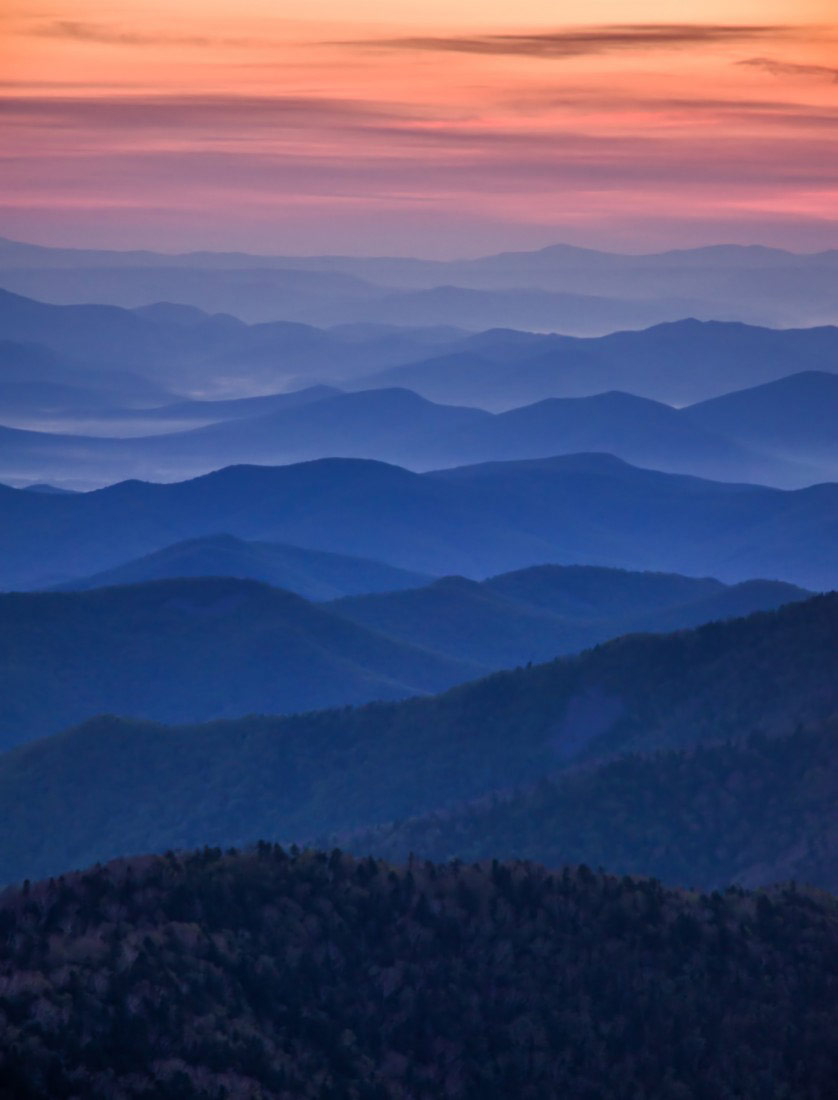
\includegraphics[scale=0.4]{photo}

\section{Tables}

\begin{center} % This do block centered
    \begin{tabular}{ |c|c|c }
        \hline
        something text №1 | something text №2 | something text №3 \\
        something text №4 | something text №5 | something text №6 \\
        something text №7 | something text №8 | something text №9 \\
        \hline
    \end{tabular}
\end{center}

\section{Mathematics}

\title{Euler integrals:}

$\displaystyle\Gamma(x) = \int_{0}^{\infty} z^{x-1} \mathrm{e}^{-z} \mathrm{d}z$

$\displaystyle B(\alpha, \beta) = \int_{0}^{1} x^{\alpha - 1} (1 - x)^{\beta - 1}\mathrm{d}x$

\end{document}
